%
% Template Laporan Skripsi/Thesis 
%
% @author  Andreas Febrian, Lia Sadita 
% @version 1.03
%
% Dokumen ini dibuat berdasarkan standar IEEE dalam membuat class untuk 
% LaTeX dan konfigurasi LaTeX yang digunakan Fahrurrozi Rahman ketika 
% membuat laporan skripsi. Konfigurasi yang lama telah disesuaikan dengan 
% aturan penulisan thesis yang dikeluarkan UI pada tahun 2008.
%

%
% Tipe dokumen adalah report dengan satu kolom. 
%
\documentclass[12pt, a4paper, onecolumn, oneside, final]{report}

% Load konfigurasi LaTeX untuk tipe laporan thesis
\usepackage{uithesis}
\usepackage{natbib}
\usepackage{import}
% Load konfigurasi khusus untuk laporan yang sedang dibuat
%-----------------------------------------------------------------------------%
% Informasi Mengenai Dokumen
%-----------------------------------------------------------------------------%
% 
% Judul laporan. 
\var{\judul}{Pembentukan Web}
% 
% Tulis kembali judul laporan, kali ini akan diubah menjadi huruf kapital
\Var{\Judul}{JUDUL SESUATU BANGET \f{ENGLISH} MIRING JUGA}
% 
% Tulis kembali judul laporan namun dengan bahasa Ingris
\var{\judulInggris}{Sesuatu Banget in English}

% 
% Tipe laporan, dapat berisi Skripsi, Tugas Akhir, Thesis, atau Disertasi
\var{\type}{Skripsi}
% 
% Tulis kembali tipe laporan, kali ini akan diubah menjadi huruf kapital
\Var{\Type}{Skripsi}
% 
% Tulis nama penulis 
\var{\penulis}{Andri Kurniawan}
% 
% Tulis kembali nama penulis, kali ini akan diubah menjadi huruf kapital
\Var{\Penulis}{Andri Kurniawan}
% 
% Tulis NPM penulis
\var{\npm}{1306382064}
% 
% Tuliskan Fakultas dimana penulis berada
\Var{\Fakultas}{Ilmu Komputer}
\var{\fakultas}{Ilmu Komputer}
% 
% Tuliskan Program Studi yang diambil penulis
\Var{\Program}{Ilmu Komputer}
\var{\program}{Ilmu Komputer}
\var{\programEng}{Computer Science}
% 
% Tuliskan tahun publikasi laporan
\Var{\bulanTahun}{Juni 2017}
% 
% Tuliskan gelar yang akan diperoleh dengan menyerahkan laporan ini
\var{\gelar}{Sarjana Ilmu Komputer}
% 
% Tuliskan tanggal pengesahan laporan, waktu dimana laporan diserahkan ke 
% penguji/sekretariat
\var{\tanggalPengesahan}{5 Juni 2017} 
% 
% Tuliskan tanggal keputusan sidang dikeluarkan dan penulis dinyatakan 
% lulus/tidak lulus
\var{\tanggalLulus}{5 Juli 2017}
% 
% Tuliskan pembimbing 
\var{\pembimbing}{Dr. Ade Azurat}
% 
% Alias untuk memudahkan alur penulisan paa saat menulis laporan
\var{\saya}{Penulis}

%-----------------------------------------------------------------------------%
% Judul Setiap Bab
%-----------------------------------------------------------------------------%
% 
% Berikut ada judul-judul setiap bab. 
% Silahkan diubah sesuai dengan kebutuhan. 
% 
\Var{\kataPengantar}{Kata Pengantar}
\Var{\babSatu}{Pendahuluan}
\Var{\babDua}{Tinjauan Pustaka}
\Var{\babTiga}{Desain}
\Var{\babEmpat}{Implementasi}
\Var{\babLima}{Hasil}
\Var{\babEnam}{Penutup}

% Daftar pemenggalan suku kata dan istilah dalam LaTeX
%
% Hyphenation untuk Indonesia 
%
% @author  Andreas Febrian
% @version 1.00
% 
% Tambahkan cara pemenggalan kata-kata yang salah dipenggal secara otomatis 
% oleh LaTeX. Jika kata tersebut dapat dipenggal dengan benar, maka tidak 
% perlu ditambahkan dalam berkas ini. Tanda pemenggalan kata menggunakan 
% tanda '-'; contoh:
% menarik
%   --> pemenggalan: me-na-rik
%

\hyphenation{
    % alphabhet A
    a-na-li-sa a-tur 
    a-pli-ka-si 
    % alphabhet B
    ba-ngun-an 
    be-be-ra-pa 
    ber-ge-rak
    ber-ke-lan-jut-an 
    ber-pe-nga-ruh 
    % alphabhet C
    ca-ri
    % alphabhet D
    di-ban-ding-kan
    di-de-fi-ni-si-kan
    di-ha-rap-kan
    di-ka-te-go-ri-kan
    di-mi-li-ki-nya
    di-se-rah-kan
    di-sim-pan di-pim-pin de-ngan da-e-rah di-ba-ngun da-pat di-nya-ta-kan 
    di-sim-bol-kan di-pi-lih di-li-hat de-fi-ni-si
    di-se-su-ai-kan
    % alphabhet E
    e-le-men
    e-ner-gi eks-klu-sif
    % alphabhet F
    fa-si-li-tas
    % alphabhet G
    ga-bung-an ge-rak
    % alphabhet H
    ha-lang-an
    he-te-ro-gen
    % alphabhet I
    i-ngin
    % alphabhet J
    % alphabhet K
    ke-hi-lang-an
    ku-ning 
    kua-li-tas ka-me-ra ke-mung-kin-an ke-se-pa-ham-an
    ke-te-pat-an
    kon-fi-gu-ra-si
    % alphabhet L
    ling-kung-an
    % alphabhet M
    me-min-ta
    me-mo-del-kan
    me-mo-ri
    men-de-fi-ni-si-kan
    me-neng-ah
    meng-a-tas-i me-mung-kin-kan me-nge-na-i me-ngi-rim-kan 
    meng-u-bah meng-a-dap-ta-si me-nya-ta-kan mo-di-fi-ka-si
    meng-a-tur
    meng-au-to-ma-si
    meng-a-ko-mo-da-si
    me-ngo-rek-si
    % alphabhet N
    nya-ta non-eks-klu-sif
    % alphabhet O
    % alphabhet P
    pa-ra-lel
    peng-ala-mat-an
    pen-ting
    penga-da-an
	pe-nye-rap-an 
	pe-ngon-trol
    pe-mo-del-an
    pe-ran  pe-ran-an-nya
    pe-rin-tah
    pem-ba-ngun-an pre-si-den pe-me-rin-tah prio-ri-tas peng-am-bil-an 
    peng-ga-bung-an pe-nga-was-an pe-ngem-bang-an 
    pe-nga-ruh pa-ra-lel-is-me per-hi-tung-an per-ma-sa-lah-an 
    pen-ca-ri-an peng-struk-tur-an
    pe-ner-bang-an
    pro-se-sor
    % alphabhet Q
    % alphabhet R
    ran-cang-an
    % alphabhet S
    se-dang-kan
    se-ring
    si-mu-la-si sa-ngat    
    % alphabhet T
    te-ngah
    ter-da-pat
    % alphabhet U
    u-sa-ha
    % alphabhet V
    % alphabhet W
    % alphabhet X
    % alphabhet Y
    % alphabhet Z
    % special
}
% Daftar istilah yang mungkin perlu ditandai 
%
% @author  Andreas Febrian
% @version 1.00
% 
% Mendaftar seluruh istilah yang mungkin akan perlu dijadikan 
% italic atau bold pada setiap kemunculannya dalam dokumen. 
% 

\var{\license}{\f{Creative Common License 1.0 Generic}}
\var{\bslash}{$\setminus$}


%\usepackage[backend=bibtex]{biblatex}
%\addbibresource{bib.bib}

% Awal bagian penulisan laporan
\begin{document}
%
% Sampul Laporan
%
% Sampul Laporan

%
% @author  unknown
% @version 1.01
% @edit by Andreas Febrian
%

\begin{titlepage}
    \begin{center}    
        \begin{figure}
            \begin{center}
                
\includegraphics[width=2.5cm]{pics/makara.png}
            \end{center}
        \end{figure}    
        \vspace*{0cm}
        \bo{
        	UNIVERSITAS INDONESIA\\
        }
        
        \vspace*{1.0cm}
        % judul thesis harus dalam 14pt Times New Roman
        \bo{\Judul} \\[1.0cm]

        \vspace*{2.5 cm}    
        % harus dalam 14pt Times New Roman
        \bo{\Type}

        \vspace*{3 cm}       
        % penulis dan npm
        \bo{\Penulis} \\
        \bo{\npm} \\

        \vspace*{5.0cm}

        % informasi mengenai fakultas dan program studi
        \bo{
        	FAKULTAS \Fakultas\\
        	PROGRAM STUDI \Program \\
        	DEPOK \\
        	\bulanTahun
        }
    \end{center}
\end{titlepage}


%
% Gunakan penomeran romawi
\pagenumbering{roman}

%
% load halaman judul dalam
\addChapter{HALAMAN JUDUL}
%
% Halaman Judul Laporan 
%
% @author  unknown
% @version 1.01
% @edit by Andreas Febrian
%

\begin{titlepage}
    \begin{center}\begin{figure}
            \begin{center}
                
\includegraphics[width=2.5cm]{pics/makara.png}
            \end{center}
        \end{figure}    
        \vspace*{0cm}
        \bo{
        	UNIVERSITAS INDONESIA\\
        }
        
        \vspace*{1.0cm}
        % judul thesis harus dalam 14pt Times New Roman
        \bo{\Judul} \\[1.0cm]

        \vspace*{2.5 cm}    
        % harus dalam 14pt Times New Roman
        \bo{\Type} \\
        % keterangan prasyarat
        \bo{Diajukan sebagai salah satu syarat untuk memperoleh gelar \\
        \gelar}\\

        \vspace*{3 cm}       
        % penulis dan npm
        \bo{\Penulis} \\
        \bo{\npm} \\

        \vspace*{5.0cm}

        % informasi mengenai fakultas dan program studi
        \bo{
        	FAKULTAS \Fakultas\\
        	PROGRAM STUDI \Program \\
        	DEPOK \\
        	\bulanTahun
        }
    \end{center}
\end{titlepage}

%
% setelah bagian ini, halaman dihitung sebagai halaman ke 2
\setcounter{page}{2}

% sementara ga usah
% load halaman pengesahan
%\addChapter{LEMBAR PERSETUJUAN}
%%
% Halaman Pengesahan
%
% @author  Andreas Febrian
% @author  Ardhi Putra Pratama
% @version 1.1
%

\chapter*{HALAMAN PERSETUJUAN}

\vspace*{0.2cm}
\noindent 

\noindent
\begin{tabular}{l l p{11cm}}
	\bo{Judul}&: & \judul \\ 
	\bo{Nama}&: & \penulis \\
	\bo{NPM}&: & \npm \\
\end{tabular} \\

\vspace*{1.2cm}


\noindent\begin{minipage}[b]{0.6\hsize}
  \raggedright
  Laporan \type~ini telah diperiksa dan disetujui.\\[0.3cm]
  
  \tanggalPengesahan \\[2cm]
  
  \underline{\pembimbing}\\[0.1cm]
  Pembimbing \type
\end{minipage}
\hfill
\begin{minipage}[b]{0.4\hsize}
  \raggedleft
  .\\[2cm]
  \underline{\pembimbingdua}\\[0.1cm]
  Pembimbing \type
\end{minipage}

\newpage
%
% load halaman orisinalitas 
\addChapter{LEMBAR PERNYATAAN ORISINALITAS}
%
% Halaman Orisinalitas
%
% @author  Andreas Febrian
% @version 1.01
%

\chapter*{\uppercase{halaman pernyataan orisinalitas}}
\vspace*{2cm}

\begin{center}
	\bo{\type~ini adalah hasil karya saya sendiri, \\ 
	dan semua sumber baik yang dikutip maupun dirujuk \\
	telah saya nyatakan dengan benar.} \\
	\vspace*{2.6cm}
	
	\begin{tabular}{l c l}
	\bo{Nama} & : & \bo{\penulis} \\
	\bo{NPM} & : & \bo{\npm} \\ 
	\bo{Tanda Tangan} & : & \\
	& & \\
	& & \\
	\bo{Tanggal} & : & \bo{\tanggalPengesahan} \\	
	\end{tabular}
\end{center}

\newpage
%
%
\addChapter{LEMBAR PENGESAHAN}
%
% Halaman Pengesahan Sidang
%
% @author  Andreas Febrian, Andre Tampubolon 
% @version 1.02
%

\chapter*{HALAMAN PENGESAHAN}

\vspace*{0.4cm}
\noindent 

\noindent
\begin{tabular}{ll p{9cm}}
	\type~ini diajukan oleh&: & \\
	Nama&: & \penulis \\
	NPM&: & \npm \\
	Program Studi&: & \program \\
	Judul \type&: & \judul \\
\end{tabular} \\

\vspace*{1.0cm}

\noindent \bo{Telah berhasil dipertahankan di hadapan Dewan Penguji 
dan diterima sebagai bagian persyaratan yang diperlukan untuk 
memperoleh gelar \gelar~pada Program Studi \program, Fakultas 
\fakultas, Universitas Indonesia.}\\[0.2cm]

\begin{center}
	\bo{DEWAN PENGUJI}
\end{center}

\vspace*{0.3cm}

\begin{tabular}{l l l l }
	& & & \\
	Pembimbing&: & \pembimbing & (\hspace*{3.0cm}) \\
	& & & \\
	Penguji&: & Penguji 1 & (\hspace*{3.0cm}) \\
	& & & \\
	Penguji&: & Penguji 2 & (\hspace*{3.0cm}) \\
\end{tabular}\\

\vspace*{2.0cm}

\begin{tabular}{ll l}
	Ditetapkan di&: & Depok\\
	Tanggal&: & \tanggalLulus \\
\end{tabular}


\newpage
%
%
\addChapter{\kataPengantar}
%-----------------------------------------------------------------------------%
\chapter*{\kataPengantar}
%-----------------------------------------------------------------------------%
Segala puji dan syukur penulis ucapkan atas kehadirat Allah SWT, Tuhan Yang Maha Esa, karena atas rahmat dan karunia-Nya penulis dapat menyelesaikan skripsi yang berjudul "\judul". Pada kesempatan ini penulis ingin mengucapkan terima kasih kepada seluruh pihak yang telah membantu dan mendukung penulis selama proses pengerjaan skripsi ini, dimana berkat dukungan dan doa mereka skripsi ini dapat diselesaikan.

Penulisan skripsi ini ditujukan untuk memenuhi salah satu syarat untuk menyelesaikan pendidikan pada Program \gelar, Universitas Indonesia. Penulis sadar bahwa dalam perjalanan perkuliahan hingga penulisan skripsi ini, penulis tidak sendirian. Penulis ingin berterima kasih kepada pihak-pihak berikut :

\begin{enumerate}
\item Bapak Ade Azurat selaku dosen pembimbing tugas akhir yang telah meluangkan waktunya sepanjang semester ini untuk dapat memberikan arahan, kritik dan saran kepada penulis agar dapat menyelesaikan proses pengerjaan skripsi ini.
\item Bapak Drs. Lim Yohanes Stefanus M.Math., Ph.D selaku dosen pembimbing akademis penulis yang selalu membimbing, memberi masukan dan membantu penulis selama masa perkuliahan.
\item Drs. H. Zulhaspan, MM dan Hj. Masreni Nasution selaku orangtua dari penulis serta Anita Putri dan Akbar Syarif selaku saudara dari penulis yang selalu mendoakan, mendukung serta menjadi motivasi penulis dalam mengerjakan skripsi ini.
\item Kak Afifun yang telah memberikan banyak masukan dan menjadi teman untuk berdiskusi terkait hal teknis selama pengerjaan skripsi ini.
\item Bu Maya, Kak Iis, Kak Niken serta teman-teman Lab RSE lainnya yang turut memberikan masukan dan bantuan kepada penulis.
\item Nabila Akiti Hara selaku pacar dari penulis yang selalu memberikan motivasi dan mendukung penulis selama pengerjaan skripsi serta menemani penulis melalui aplikasi \textit{facetime}.
\item Teman-teman PI BPH IMMM UI (Fadhil, Titto, Fandika, Mawan, Dodo, Okky, Devi, Rara, Ami, Rizky, Ime, Popo, Ilham) yang selalu menghibur penulis kala jenuh dalam mengerjakan skripsi dan seluruh keluarga IMMMSU UI yang telah menjadi keluarga bagi penulis selama masa perkuliahan.
\item Arief Radityo, Arsi Alhafis, dan M. Gibran yang selalu menjadi teman untuk bermain maupun belajar bagi penulis serta membantu penulis selama perkuliahan.
\item Sahabat-sahabat PPN (Abi, Budi, Cia, Dana, Erwin, Fakhry, Irene, Fadly, Fani, Mawan, Mutia, Sufi, Ulup) yang selalu menjadi penghibur bagi penulis setiap saat.
\item Teman-teman CornedIn (Arsi, Zaki, Dimas, Ilham) yang merupakan teman-teman perjuangan untuk proyekan yang mengajarkan banyak hal terkait teknikal kepada penulis.
\item Kelompok PPL B1 (Akbar, Dimas, Emon, Fajrin, Fathin), Kelompok PPL B2 (Gilang, Falah, Fatah, Nanda, Hamdan) dan Kelompok PPL B3 (Brigita, Gentur, Kowan, Riscel, Muthy) serta Kak Naya yang telah menemani penulis selama satu semester khususnya hari Rabu dan memberikan penulis pandangan baru mengenai \textit{scrum master}.
\end{enumerate}

Akhir kata, penulis berharap semoga Allah SWT dapat membalas kebaikan yang diberikan oleh orang-orang terdekat penulis dan penulis berharap karya yang penulis buat dapat membantu dan bermanfaat bagi pengembangan ilmu pengetahuan selanjutnya.

\vspace*{0.1cm}
\begin{flushright}
Depok, 5 Juni 2017\\[0.1cm]
\vspace*{1cm}
\penulis

\end{flushright}
%
%
\addChapter{LEMBAR PERSETUJUAN PUBLIKASI ILMIAH}
% 
% @author  Andre Tampubolon, Andreas Febrian
% @version 1.01
% 

\chapter*{\uppercase{Halaman Pernyataan Persetujuan Publikasi Tugas Akhir untuk Kepentingan Akademis}}

\vspace*{0.2cm}
\noindent 
Sebagai sivitas akademik Universitas Indonesia, saya yang bertanda 
tangan di bawah ini:
\vspace*{0.4cm}


\begin{tabular}{p{4.2cm} l p{6cm}}
	\bo{Nama} & : & \penulis \\ 	
	\bo{NPM} & : & \npm \\
	\bo{Program Studi} & : & \program\\	
	\bo{Fakultas} & : & \fakultas\\
	\bo{Jenis Karya} & : & \type \\
\end{tabular}

\vspace*{0.6cm}
\noindent demi pengembangan ilmu pengetahuan, menyetujui untuk memberikan 
kepada Universitas Indonesia \bo{Hak Bebas Royalti Noneksklusif 
(Non-exclusive Royalty Free Right)} atas karya ilmiah saya yang berjudul:
\begin{center}
	\judul
\end{center}
beserta perangkat yang ada (jika diperlukan). Dengan Hak Bebas Royalti 
Noneksklusif ini Universitas Indonesia berhak menyimpan, 
mengalihmedia/formatkan, mengelola dalam bentuk pangkalan data 
(\f{database}), merawat, dan memublikasikan tugas akhir saya selama 
tetap mencantumkan nama saya sebagai penulis/pencipta dan sebagai 
pemilik Hak Cipta. \\

\noindent Demikian pernyatan ini saya buat dengan sebenarnya.

\begin{center}
	\vspace*{0.8cm}
	\begin{tabular}{lll}
		Dibuat di&: & Depok \\
		Pada tanggal&: & \tanggalPengesahan \\
	\end{tabular}\\

	\vspace*{0.2cm}
	Yang menyatakan \\
	\vspace*{2cm}
	(\penulis)
\end{center}

\newpage


%
% 
\singlespacing
\addChapter{ABSTRAK}
%
% Halaman Abstrak
%
% @author  Andreas Febrian
% @version 1.00
%

\chapter*{Abstrak}

\vspace*{0.2cm}

\noindent \begin{tabular}{l l p{10cm}}
	Nama&: & \penulis \\
	Program Studi&: & \program \\
	Judul&: & \judul \\
\end{tabular} \\ 

\vspace*{0.5cm}

\noindent 
\\ Pembuatan web semantik yang belum umum dan susah, menjadikan web semantik belum populer saat ini. Padahal dengan menggunakan web semantik, informasi-informasi yang ada pada web dapat diolah secara langsung oleh komputer. Penelitian terus dilakukan untuk memudahkan pembuatan web semantik dimana salah satunya adalah zotonic. Zotonic merupakan salah satu web \textit{framework} yang berbasis semantik. Pada penelitian sebelumnya telah dikembangkan zotonic yang dapat menerima ontologi sebagai masukan untuk pembentukan struktur webnya. Namun, karena ontologi tidak mengandung \textit{business logic}, maka diperlukan mekanisme untuk menghubungkan ontologi dengan ABS \textit{microservices} agar \textit{business logic} pada Zotonic dapat bersifat dinamis berdasarkan kebutuhkan. Penelitian ini membahas bagaimana ontologi dan \textit{web service} yang dihasilkan oleh ABS \textit{microservices} dapat diintegrasikan. Hal ini berguna agar dapat menciptakan beberapa web pada zotonic yang memiliki struktur yang sama namun memiliki \textit{business logic} yang berbeda. Tahapan dari penelitian ini adalah melakukan rancangan terhadap integrasi yang akan dilakukan dan implementasi \textit{adaptor} yang digunakan sebagai penghubung antara ontologi dan \textit{web services}. Pada akhir penelitian ini, dilakukan ujicoba untuk melihat hasil dari implementasi yang telah dilakukan.

\vspace*{0.2cm}

\noindent Kata Kunci: \\ 
\noindent ABS, \textit{Adaptor}, SPL, \textit{Web Service}, Zotonic\\ 

\newpage
%
%
%
% Halaman Abstract
%
% @author  Andreas Febrian
% @version 1.00
%

	\chapter*{ABSTRACT}

\vspace*{0.2cm}

\noindent \begin{tabular}{l l p{11.0cm}}
	Name&: & \penulis \\
	Program&: & \programEng \\
	Title&: & \judulInggris \\
\end{tabular} \\ 

\vspace*{0.5cm}

\noindent 
\\ Making semantic web is not yet common and difficult, making semantic web not yet popular at this time. Whereas, by using semantic web, the information available on the web can be processed directly by computer. Research continues to be done to facilitate the manufacture of semantic web where one of them is zotonic. Zotonic is one of the semantic-based web frameworks. In the previous research has been developed zotonic that can accept ontology as input for the formation of web structure. However, since ontology does not contain business logic, a mechanism for connecting ontology with ABS microservices is required so that business logic on Zotonic can be dynamic based on need. This study discusses how the ontology and web services produced by ABS microservices can be integrated. This is useful in order to create multiple webs on zotonic that have the same structure but have different business logic. The stages of this research is to design the integration that will be done and the implementation of the adaptor used as a liaison between ontology and web services. At the end of this study, a trial is conducted to see the results of the implementation that has been done.

\vspace*{0.2cm}

\noindent Keywords: \\ 
\noindent ABS, Adaptor, SPL, Web Service, Zotonic\\

\newpage

%
% Daftar isi, gambar, dan tabel
%
\tableofcontents
\clearpage
\listoffigures
\clearpage
\listoftables
\clearpage
\lstlistoflistings
\clearpage

%
% Gunakan penomeran Arab (1, 2, 3, ...) setelah bagian ini.
%
\pagenumbering{arabic}

%
%
%
\onehalfspacing
%-----------------------------------------------------------------------------%
\chapter{\babSatu}
%-----------------------------------------------------------------------------%

Bab ini menjelaskan latar belakang permasalahan, perumusan masalah, tujuan penelitian ini dilakukan, ruang lingkup penelitian serta sistematika penulisan.

%-----------------------------------------------------------------------------%
\section{Latar Belakang}
%-----------------------------------------------------------------------------%

Penggunaan \textit{web} sebagai sarana untuk berbagi informasi pada saat ini sangat tinggi. Namun, tidak banyak orang yang mampu mengembangkan web serta tidak adanya anggaran untuk pembuatan \textit{web} menjadi masalah tersendiri terutama bagi organisasi non-profit. Selain itu, banyaknya informasi yang tersebar di \textit{web} saat ini hanya sebatas informasi saja yang tidak dapat diolah. Hal ini karena informasi-informasi tersebut tidak memiliki hubungan yang terstruktur dan hanya didesain untuk manusia saja sehingga program komputer tidak dapat mengolah informasi tersebut \citep{berners.semantic}.

Selain permasalahan informasi yang tidak dapat diolah oleh komputer, permasalahan lainnya adalah \textit{web} yang ada saat ini kebanyakan memiliki fitur yang sama. Namun, dalam pembuatannya setiap \textit{web} hanya didesain khusus untuk pembuatan satu \textit{web} saja. Tentu saja hal ini dapat dibantu dengan menerapkan paradigma \textit{software product line} dimana \textit{software product line} dapat menghemat biaya produksi, mempercepat waktu produksi ke pasar serta lebih menjadi kualitas dari produk yang dihasilkan \citep{book.sple}.

Pada tahun 2001, \cite{berners.semantic} menemukan sebuah teknologi yang dinamakan \textit{web} semantik, dimana \textit{web} semantik akan membuat sebuah struktur untuk informasi yang terdapat pada \textit{web} sehingga informasi-informasi tersebut dapat diolah oleh program komputer \citep{berners.semantic}. Menurut Rob McCool, Format yang kompleks dan pengguna harus mengorbankan kemudahan ekspresivitas serta membayar biaya yang besar untuk translasi dan perawatan menjadi alasan kenapa \textit{web} semantic tidak akan pernah diadopsi publik secara luas \citep{pragmatic.web}.

Untuk mempermudah proses pembuatan \textit{web} semantik, maka diciptakan \textit{web} pragmatis dimana tujuannya adalah meningkatkan kolaborasi manusia untuk lebih efektif dengan teknologi yang tepat seperti sistem untuk negosiasi ontologi, interaksi bisnis yang terdapat pada ontologi, dan untuk membangun ontologi pragmatis pada praktik masyarakat \citep{pragmatic.web}. Sehingga \textit{web} pragmatis dapat melengkapi \textit{web} semantik untuk berkolaborasi dan meningkatkan kualitas pada level masyarakat.Salah satu perkembangan \textit{web} semantik pragmatis adalah Zotonic, yaitu sebuah framework sekaligus Content Management System (CMS) yang dibangun di atas bahasa pemrograman erlang dimana Zotonic telah mengadopsi konsep \textit{web} semantik. Kehadiran Zotonic sendiri diharapkan dapat meningkatkan pemanfaatan \textit{web} semantik dalam proses pembuatan \textit{web}. sehingga infomasi yang berada pada \textit{web} yang dibuat dapat langsung diolah oleh komputer. Tetapi, pengembang perlu mendefinisikan semantik yang akan mereka buat terlebih dahulu sebelum mereka mengembangkannya dalam Zotonic untuk menciptakan sebuah konsistensi. Namun hal ini tentu saja menghambat proses pengembangan karena pengembang membutuhkan waktu yang lebih lama untuk proses translasi dari semantik ke Zotonic.

Untuk membantu para pengembang dalam mentranslasikan semantik ke dalam Zotonic, pada tahun 2016 terdapat sebuah penelitian terkait pembentukan otomatis aplikasi \textit{web} dengan masukan berupa ontologi, yaitu penelitian terkait pemetaan ontologi yang dihasilkan semantik ke dalam struktur Zotonic \citep{bravyto}. Namun, pada penelitian tersebut pembentukan \textit{business logic} dari \textit{web} yang dibentuk masih secara manual. Hal ini dikarenakan pada ontologi tidak terdapat \textit{business logic} sehingga tidak dapat secara otomatis. \textit{Business logic} tersebut dapat diperoleh dari ABS \textit{microservices} seperti pada \pic~\ref{fig:roadmapbab1}.

\begin{figure}
	\centering
	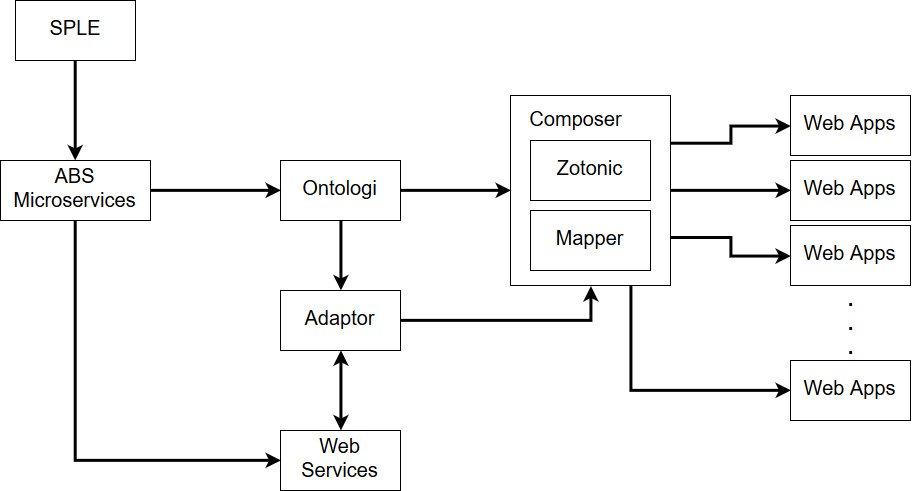
\includegraphics[width=1\textwidth]
	{pics/roadmapbab1.jpg}
	\caption{\textit{Roadmap} pembentukan \textit{web} berbasis semantik}
	\label{fig:roadmapbab1}
\end{figure}
\vspace{-0.3cm}

Dengan memanfaatkan ABS \textit{microservices} yang dihasilkan dari SPLE, maka tidak hanya membuat sebuah \textit{web} berbasis semantik saja tetapi Zotonic yang dihasilkan nantinya dapat membuat beberapa \textit{web} berbasis semantik yang memiliki struktur yang sama yang berasal dari ontologi dan \textit{business logic} yang dapat disesuaikan dengan kebutuhannya. Oleh karena itu, penting untuk dilakukan penelitian mengenai bagaimana cara menghubungkan ontologi tersebut dengan \textit{web services} pada Zotonic agar lebih memudahkan dan lebih efisien dalam pembuatan \textit{web}.
%-----------------------------------------------------------------------------%
\section{Perumusan Masalah}
%-----------------------------------------------------------------------------%
Berdasarkan latar belakang tersebut, penelitian ini akan mencoba untuk menjawab beberapa pertanyaan penelitian, yaitu
\begin{enumerate}
\item Bagaimana proses integrasi ontologi kepada \textit{web service}?
\item Apakah dapat dikembangkan sebuah program \textit{adaptor} yang akan melakukan integrasi ontologi dan \textit{web service} secara otomatis?
\end{enumerate}
%-----------------------------------------------------------------------------%
\section{Tujuan Penelitian}
%-----------------------------------------------------------------------------%
Tujuan dari penelitian ini adalah untuk mengembangkan sebuah program yang dapat menghubungkan antara \textit{web services} dan Zotonic sehingga proses pembuatan \textit{site} pada Zotonic dapat memiliki tingkat adaptasi yang baik terhadap perubahan yang terjadi. Harapannya melalui program yang dibuat, pengembang dapat tetap fokus untuk \textit{maintain} data dan mengembangkan aplikasi, karena data sudah terjadi melalui ontologi.

%-----------------------------------------------------------------------------%
\section{Ruang Lingkup Penelitian}
%-----------------------------------------------------------------------------%

Ruang lingkup penelitian ini antara lain:
\begin{enumerate}
\item Analisis pemetaan \textit{adaptor} untuk menghubungkan antara ontologi dan \textit{web service}.
\item Perancangan sistem yang dapat menghubungkan antara ontologi dan \textit{web service} melalui Zotonic.
\item \textit{Refactoring} pembuatan \textit{business logic} yang sudah ada dengan memanfaatkan sistem yang dibuat.
\end{enumerate}

%-----------------------------------------------------------------------------%
\section{Sistematika Penulisan}
%-----------------------------------------------------------------------------%
Sistematika penulisan laporan adalah sebagai berikut:
\begin{itemize}
	\item Bab 1 \babSatu
	
	Bab 1 berisi tentang informasi terkait penelitian yang dilakukan oleh penulis, dimana bab ini terdiri atas 5 subbab, yaitu latar belakang, perumusan masalah yang akan diteliti oleh penulis, tujuan penelitian, ruang lingkup penelitian serta sistematika penulisan.\\
	\item Bab 2 \babDua
	
	Bab 2 berisi mengenai penjelasan terkait ontologi, \textit{web} \textit{framewok} berbasis semantic: Zotonic, dan \textit{software product line}.\\
	\item Bab 3 \babTiga 
	
	Bab 3 berisi penjelasan mengenai rancangan dari sistem yang akan diimplementasikan, dimana bab ini terdiri atas 3 subbab, yaitu rancangan integrasi ontologi dan \textit{web service}, rancangan \textit{web service} serta rancangan \textit{adaptor}.\\
	
	\item Bab 4 \babEmpat
	
	Bab 4 berisi penjelasan mengenai impelementasi yang dilakukan oleh penulis untuk membuat \textit{adaptor}. \\
	
	\item Bab 5 \babLima	
	
	Bab 5 berisi perubahan yang terjadi setelah eksperimen dan hasil uji coba eksperimen yang telah dilakukan oleh penulis. \\
	
	\item Bab 6 \babEnam
	
	Bab 6 berisi kesimpulan yang didapat dari penelitian serta saran yang diajukan untuk penelitian berikutnya.
\end{itemize}
%-----------------------------------------------------------------------------%
\chapter{\babDua}
%-----------------------------------------------------------------------------%
Bab ini berisi tentang tinjauan pustaka yang terkait dengan penelitian. Bab ini akan menjelaskan mengenai ontologi, zotonic, dan \textit{software product line}.
%-----------------------------------------------------------------------------%
\section{Ontologi}
%-----------------------------------------------------------------------------%
	
Ontologi merupakan bagian yang paling mendasar dari web semantik. Ontologi
adalah sebuah deskripsi formal yang eksplisit tentang kelas (domain atau disebut juga sebagai \textit{concepts}), relasi, dan \textit{property} dari setiap domain, yang biasanya telah terdefinis secara baik \citep{hopkins_powell_2015}. Menurut \cite{ontologydevelopment}, pengembangan ontologi perlu dilakukan karena beberapa alasan berikut ini.

\begin{enumerate}
\item Berbagi pemahaman umum terkait struktur dari informasi diantara manusia ataupun \textit{software agents}.
\item Menggunakan kembali pengetahuan dari kelas.
\item Membuat asumsi terkait kelas tersampaikan secara eksplisit.
\item Memisahkan pengetahuan tentang kelas dari pengetahuan secara operasional.
\item Menganalisa pengetahuan tentang kelas.
\end{enumerate}

Berbagi pemahaman umum terkait struktur dari informasi merupakan satu dari beberapa tujuan utama pada pengembangan ontologi \citep{paper.gruber}. Dengan adanya pemahaman terkait struktur dari informasi yang diperoleh, sebuah \textit{software agents} dapat mengekstrak dan mengumpulkan informasi yang diperoleh dari berbagai layanan yang berbeda namun menggunakan dasar ontologi yang sama. Selain dapat memperoleh informasi, dengan menggunakan struktur ontologi yang cenderung sama maka sebuah ontologi dapat digunakan kembali untuk kasus yang cenderung sama atau mirip sehingga dapat melakukan penghematan dana maupun waktu.

Ontologi terdiri dari beberapa komponen yaitu kelas, atribut, relasi. Ketika membuat ontologi, kelas merupakan komponen yang harus dibuat pertama kali karena kelas merupakan komponen utama dari ontologi. Kelas atau disebut juga domain, merupakan kumpulan data pada ontologi yang memiliki sebuah nama yang deskriptif untuk menggambarkan data tersebut. Salah satu contoh dari kelas adalah sebagai berikut

\begin{figure}
	\centering
	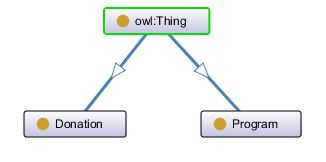
\includegraphics[width=0.7\textwidth]
	{pics/domain.jpg}
	\caption{Contoh Kelas pada Ontologi}
	\label{fig:class}
\end{figure}
\vspace{-0.3cm}

Pada \pic~\ref{fig:class}, Program dan \textit{Donation} merupakan salah satu contoh dari kelas (disebut sebagai \textit{thing} pada \textit{software} protege). Program merupakan kumpulan data mengenai kegiatan yang dilakukan sedangkan \textit{Donation} merupakan kumpulan data mengenai donasi terhadap suatu program. Kelas Program dan \textit{Donation} membutuhkan atribut yang akan menjelaskan tentang kelas tersebut sehingga perlu didefinisikan apa yang menjadi atribut dari kelas tersebut. Pada penelitian ini, penulis menggunakan ontologi yang sudah ada yaitu ontologi \textit{charity organization} dimana kelas Program memiliki atribut name dan total sedangkan kelas \textit{Donation} memiliki atribut \textit{amount}. Pada gambar \pic~\ref{fig:class}, belum terdapat keterhubungan diantara kelas Program dan \textit{Donation} sehingga perlu membuat komponen terakhir yaitu relasi. Setiap relasi harus dapat menggambarkan keterhubungan dari kelas yang ada. Pada ontologi \textit{charity organization} yang digunakan, kelas Program dan \textit{Donation} dihubungkan menggunakan relasi \textit{Channeled through} seperti gambar berikut

\begin{figure}
	\centering
	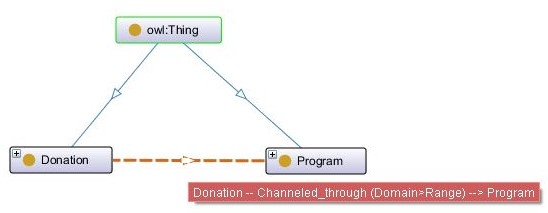
\includegraphics[width=0.9\textwidth]
	{pics/relationClass.jpg}
	\caption{Contoh Relasi pada Ontologi}
	\label{fig:relationClass}
\end{figure}
\vspace{-0.3cm}

Pada gambar \pic~\ref{fig:relationClass}, dapat dilihat bahwa kelas \textit{Donation} dan kelas Program dihubungkan oleh relasi \textit{Channeled through} yang berarti suatu donasi dapat disalurkan kepada suatu program. Relasi antar keduanya digambarkan sebagai sebuah edge pada graf ontologi. 

Selain memiliki tiga komponen yang telah disebutkan diatas, pada ontologi juga terdapat struktur hierarki yang dapat dimiliki oleh suatu kelas. Struktur hierariki ini menggambarkan tingkatan dari suatu kelas. Kelas yang memiliki tingkatan lebih tinggi biasanya merupakan kelas yang bersifat lebih umum dari kelas-kelas yang memiliki tingkatan lebih rendah dari dirinya. Sebagai contoh, kelas Hewan memiliki tingkatan yang lebih daripada kelas Mamalia dan juga kelas Reptil karena mamalia dan reptil merupakan bagian dari hewan. Hal ini dapat dilihat pada \pic~\ref{fig:subClass} dimana kelas \textit{EventualProgram} memiliki tingkatan yang lebih rendah dari kelas Program atau disebut dengan \textit{subclass}. Untuk kelas yang memiliki tingkatan yang lebih rendah dari kelas diatasnya, kelas tersebut akan mewarisi semua atribut atau properti yang terdapat pada kelas yang lebih tinggi dari dirinya. Sebagai contoh, kelas Program memiliki atribut \textit{name} dan total sehingga kelas \textit{ContinuousProgram, EventualProgram serta PeriodicProgram} akan memiliki atribut \textit{name} dan total juga.

\begin{figure}
	\centering
	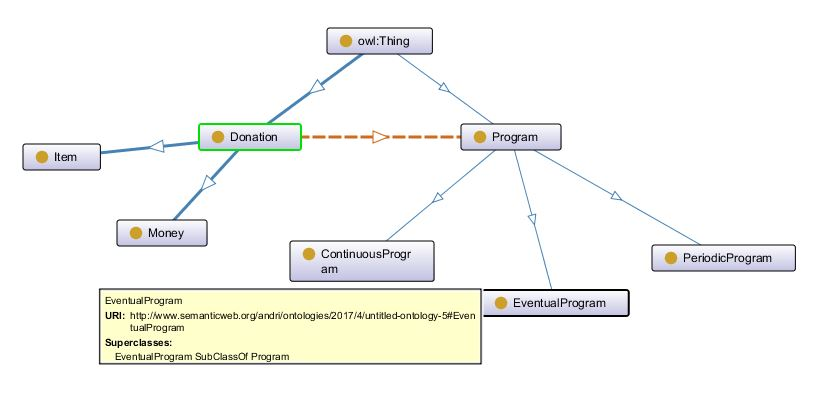
\includegraphics[width=1\textwidth]
	{pics/subClass.jpg}
	\caption{Contoh Struktur Hierarki}
	\label{fig:subClass}
\end{figure}
\vspace{-0.3cm}

Agar ontologi dapat dipahami oleh komputer, ontologi tersebut harus direpresentasikan dalam bentuk yang dapat dibaca oleh komputer salah satunya adalah OWL. \textit{Ontoloy Web Language} (OWL) merupakan versi RDFS yang memiliki kosa kata dan \textit{rules} yang lebih ketat sehingga OWL lebih mudah dipahami oleh komputer karena dapat lebih menggambarkan ontologi yang dibuat \citep{owl.overview}. Pada penelitian ini, digunakan setidaknya tiga elemen dari OWL yaitu \textit{class, datatype property} serta \textit{object property}. \textit{Class} akan menggambarkan kelas dari ontologi, \textit{datatype property} akan menggambarkan atribut dari kelas, serta \textit{object property} akan menggambarkan relasi antar suatu kelas dengan kelas lainnya.
%-----------------------------------------------------------------------------%
\section{Zotonic}
%-----------------------------------------------------------------------------%

Zotonic merupakan web yang bersifat \textit{open source}, \textit{real-time web framework}, dan sekaligus sebagai \textit{Content Management System} (CMS) yang dibangun menggunakan bahasa pemrograman erlang \citep{zotonic.overview}. Selain merupakan sebuah CMS dan \textit{framework}, Zotonic juga merupakan sebuah web server yang dapat menjalankan web langsung tanpa bantuan web server seperti Apache dan Nginx. Karena dibangun dengan bahasa pemrograman erlang, Zotonic sangat mengutamakan kecepatan.

Menurut Zotonic, kecepatan dari zotonic ini sendiri bisa mencapai 10x lebih cepat daripada CMS yang dibangun menggunakan bahasa pemrograman PHP. Hal ini berdasarkan perbandingan antara proses pembuatan halaman pada kebanyakan \textit{framework} PHP yang membutuhkan waktu 150-600 ms sedangkan pada Zotonic biasanya hanya membutuhkan waktu 10 ms atau kurang. Selain itu, Zotonic memiliki mekanisme untuk mencegah permintaan yang berbeda untuk melakukan hal yang sama pada waktu yang bersamaan. Ketika terdapat dua atau lebih permintaan datang untuk halaman yang sama, atau bagian dari halaman yang sama, maka zotonic akan melakukan pekerjaan sekali dan mengirimkan hasilnya ke semua permintaan yang masuk. Zotonic juga menyimpan data yang sering digunakan pada memori, sehingga dapat mencegah kueri yang banyak kepada database. Pada erlang, kode akan dimuat dan akan terus dimuat sampai ada perubahaan kode berikutnya sehingga hal ini dapat membuat zotonic lebih efisien dibandingkan PHP \citep{zotonic.speed}.

Zotonic juga menerapkan sistem modular. Zotonic dibuat dari lapisan kode yang umum dengan modul yang menyediakan fungsi utama lainnya. \textit{Template, actions, controllers, javascript, css, dispatch rules}, semuanya berasal dari modul. Modul dapat memperbanyak, mengubah atau bekerja sama dengan modul lainnya. Modul dapat mendefinisikan ulang \textit{template, javascript, css, actions} dan \textit{dispatch rules} dari modul lainnya.

Zotonic juga melakukan pemisahan antara model, tampilan, dan \textit{controller} atau biasa disebut MVC yang telah menjadi \textit{best practice} pada proses pembuatan web dalam waktu yang lama. Hal ini bagus untuk pemisahan tanggung jawab \citep{zotonic.mvc}. Hal ini akan memberikan kesempatan kepada \textit{programmer} dari program dan pengembang tampilan (\textit{front-ender}) untuk membuat HTML, CSS, dan lainnya sendiri berdasarkan kebutuhannya. Pengembang tampilan memiliki akses baca pada hampir semua informasi yang tersedia pada Zotonic. Pada \textit{template} dapat langsung memanggil kueri, mengambil \textit{properties} dari pages, melakukan pengecekan kunci konfigurasi, dan lainnya. Sehingga \textit{programmer} tidak butuh membuat \textit{controller} lainnya atau mengadopsi beberapa \textit{controller} untuk memberikan informasi ekstra kepada \textit{template}. Dan pengembang tampilan tidak perlu untuk menunggu \textit{programmer}. Hal ini berguna agar pengembang tampilan dapat secara langsung mengambil dan menampilkan data dari Zotonic pada \textit{template}.

Selain itu, tampilan pada zotonic dibangun menggunakan \textit{jQuery} dan CSS \textit{framework Bootstrap} yang merupakan salah satu CSS \textit{framework} yang sangat populer saat ini \citep{awwwards.css}. Selain penggunaan \textit{jQuery} dan \textit{Bootstrap}, Zotonic juga mengadopsi penggunaan ErlyDTL (\textit{Erlang implementation of the Django Template Language}). ErlyDTL digunakan agar pemuatan data dari basis data dapat dilakukan langsung dari \textit{template} yang ingin memuat data itu sendiri. Zotonic sendiri menambahkan beberapa fitur pada ErlyDTL yang diadopsi seperti untuk \textit{caching} dan \textit{template} hanya di\textit{compile} ke memori sehingga dapat mencegah masalah ketika logika internal dari \textit{template} berubah versi.

Selain itu, zotonic menawarkan fitur fleksibilitas pada model data. Hal ini karena zotonic memberikan kebebasan kepada penggunanya untuk melakukan penambahan atau pengurangan terhadap model data. Model data pada Zotonic sendiri merupakan bentuk implementasi dari web semantik. Model datanya memiliki dua konsep utama yaitu \textit{resource} dan \textit{edge} \citep{zotonic.model}. \textit{Resource} pada Zotonic biasanya disebut sebagai \textit{pages} pada halaman admin karena semua \textit{resource} yang dihasilkan pada aplikasi akan ditampilkan sebagai sebuah \textit{pages}. \textit{Resources} memiliki bagian utama yaitu mereka memiliki \textit{properties} seperti judul, ringkasan, dan isi bodi serta mereka milik dari sebuah \textit{category}.

\begin{figure}
	\centering
	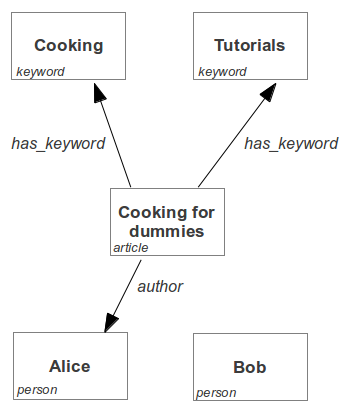
\includegraphics[width=0.6\textwidth]
	{pics/dataModel.png}
	\caption{Contoh Data Model}
	\label{fig:dataModel}
\end{figure}
\vspace{-1cm}
\begin{center}
{\small Sumber gambar: \citep{zotonic.model}}
\end{center}

Pada \pic~\ref{fig:dataModel}, blok persegi menggambarkan \textit{resource} dan panah menggambarkan \textit{edge}. Alice adalah sebuah \textit{resource} yang berkategori \textit{person}. Begitu juga halnya dengan Bob yang merupakan \textit{resource} dengan kategori \textit{person}. Hal ini menunjukkan bahwa pada Zotonic, suatu kategori dapat memiliki banyak \textit{instance} yang berupa \textit{resource}. \textit{Cooking} dan \textit{Tutorials} sama-sama merupakan \textit{resources} yang berkategori \textit{keyword} sedangan \textit{Cooking For Dummies} merupakan \textit{resource} yang berkategori \textit{article}. \textit{has\_keyword} merupakan \textit{edge} yang menunjukan hubungan antara suatu \textit{resource} dengan \textit{resource} lainnya. Hal ini dapat dilihat bahwa \textit{resource cooking for dummies} memiliki \textit{keyword} yaitu \textit{cooking} dan \textit{tutorials}. Dengan kata lain, kategori \textit{article} memiliki hubungan dengan kategori \textit{keyword} yaitu \textit{article} mempunyai \textit{keyword}. Ini sama dengan relasi yang menghubungkan suatu \textit{class} dengan \textit{class} lainnya pada ontologi. Dengan model data yang seperti ini, zotonic merupakan salah satu CMS yang menerapkan implementasi dari web semantik.
%-----------------------------------------------------------------------------%
\section{\textit{Software Product Line}}
%-----------------------------------------------------------------------------%
	\todo{Jelasin SPL itu apa.}

%-----------------------------------------------------------------------------%
\chapter{\babTiga}
%-----------------------------------------------------------------------------%

Dari permasalahan yang sudah didefinisikan, maka akan dibuat sebuah program yang akan melakukan integrasi ontologi dan \textit{web service} dengan memanfaatkan Zotonic. Sebelum memulai pembuatan program, perlu dirancang bagaimana program ini akan berjalan. Pada bab ini, akan dibahas mengenai rancangan integrasi ontologi dan \textit{web service} yang akan menggambarkan secara keseluruhan bagaimana program akan bekerja serta hal lainnya yang terhubungan dengan program dan juga mengenai rancangan adaptor yang akan menggambarkan secara dalam bagaimana program dapat mengakses \textit{web service} dan terhubung dengan ontologi.
%-----------------------------------------------------------------------------%
\section{Rancangan Integrasi Ontologi dan \textit{Web Service}}
%-----------------------------------------------------------------------------%

Agar dapat menghasilkan program yang bertujuan untuk melakukan integrasi ontologi dan \textit{web services} maka perlu dirancang secara keseluruhan bagaimana program ini akan bekerja. Sesuai dengan kebutuhan dari program, maka integrasi ini akan dilakukan pada sebuah \textit{framework} sekaligus \textit{CMS} Zotonic, yang telah dimodifikasi agar dapat menerima masukan berupa ontologi. Secara garis besar, berikut merupakan gambaran cara program akan bekerja.

\begin{figure}
	\centering
	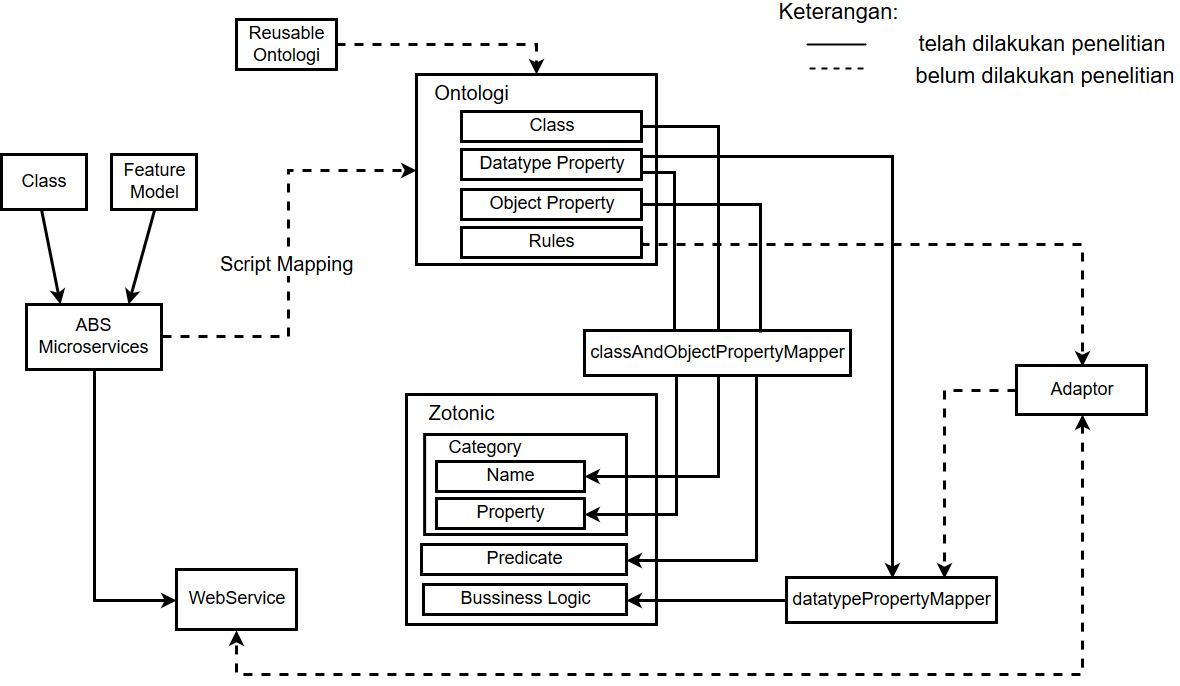
\includegraphics[width=1\textwidth]
		{pics/skripsiRoadmapNew.jpg}
	\caption{Rancangan integrasi ontologi dan web service}
	\label{fig:skripsiroadmap}
\end{figure}
\vspace{-0.3cm}

Seperti yang dapat dilihat pada \pic~\ref{fig:skripsiroadmap}, \textit{Class} dan \textit{Feature Model} akan diproses menggunakan program translasi yang akan menghasilkan ABS \textit{Microservices} dimana ini telah dilakukan penelitian sebelumnya sehingga hal ini bukan merupakan bagian dari penelitian penulis. Setelah dihasilkan sebuah ABS \textit{Microservices} dari proses translasi tersebut, maka ABS \textit{Microservices} akan menghasilkan sebuah \textit{web service} yang dapat digunakan oleh program lainnya. Dalam penelitian ini, \textit{web services} yang dihasilkan oleh ABS \textit{Microservices} akan digunakan oleh \textit{Adaptor} yang akan terhubung dengan Zotonic. Selain digunakan untuk menghasilkan sebuah \textit{web service}, ABS \textit{Microservices} akan digunakan untuk menghasilkan sebuah ontologi menggunakan sebuah \textit{script} yang akan melakukan pemetaan dari \textit{class} dan \textit{feature model} menjadi \textit{class, datatype property, object property} dan \textit{rules} pada ontologi. Untuk pemetaan ini sendiri tidak termasuk dalam penelitian ini karena penulis hanya akan menggunakan sebuah ontologi yang telah dirancang sebelumnya. Nantinya melalui proses pemetaan ini, akan dihasilkan sebuah ontologi yang bersifat \textit{reusable}.

Menggunakan ontologi yang telah dirancang sebelumnya, ontologi tersebut akan dipetakan ke dalam struktur dari zotonic yang akan digunakan. Proses pemetaan dari ontologi ke dalam zotonic ini sendiri telah dilakukan pada penelitian sebelumnya oleh Bravyto dimana setiap \textit{class} dari ontologi akan dipetakan menjadi nama dari kategori pada zotonic menggunakan \textit{script classAndObjectPropertyMapper.sh}. Selain melakukan pemetaan pada \textit{class, script} tersebut juga akan melakukan pemetaan \textit{datatype property} pada ontologi menjadi \textit{property} dari kategori pada zotonic serta pemetaan \textit{object property} pada ontologi menjadi \textit{predicate} pada zotonic. Pada penelitian tersebut, dilakukan juga pemetaan dari \textit{datatype property} menjadi \textit{business logic} menggunakan \textit{script} datatypePropertyMapper.sh.

Namun pada penelitian tersebut, pembuatan \textit{business logic} masih bersifat manual yang langsung ditaruh pada \textit{script} datatypepropertyMapper.sh. Pada penelitian ini, penulis akan membuat sebuah adaptor yang akan memanggil \textit{web service} sehingga \textit{business logic} pada zotonic akan lebih fleksibel karena memanfaatkan \textit{web service} serta memberikan kemudahan bagi \textit{developer} dalam hal melakukan modifikasi.
%-----------------------------------------------------------------------------%
\section{Rancangan \textit{Web Service}}
%-----------------------------------------------------------------------------%

	\todo{Jelasin gimana rancangan API nya.}

%-----------------------------------------------------------------------------%
\section{Rancangan \f{Adaptor}}
%-----------------------------------------------------------------------------%

Adaptor merupakan sebuah \textit{script} yang akan memanggil \textit{web service} sehingga dapat digunakan untuk melakukan pemrosesan \textit{business logic} pada zotonic. Bagaimana adaptor akan bekerja sehingga menghasilkan business logic dapat dilihat pada gambar berikut ini.

\begin{figure}
	\centering
	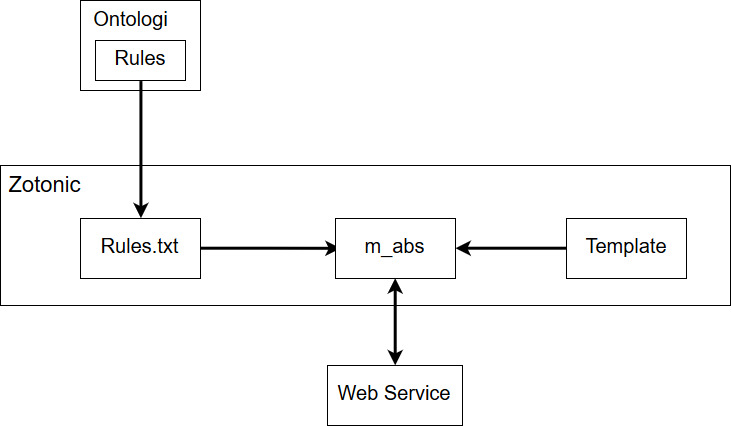
\includegraphics[width=0.7\textwidth]
		{pics/adaptor.jpg}
	\caption{Rancangan Adaptor}
	\label{fig:adaptor}
\end{figure}
\vspace{-0.3cm}

Seperti yang dapat dilihat pada \pic~\ref{fig:adaptor}, \textit{rules} yang terdapat pada ontologi akan dilakukan pemetaan menjadi tabel \textit{rules} yang akan disimpan pada file rules.txt seperti yang terdapat pada kode \ref{lst:tablerules}. Namun, proses pemetaan ini berada diluar dari topik penelitian penulis sehingga untuk keperluan penelitian ini maka penulis membuat sebuah tabel \textit{rules} secara manual untuk mengganti proses pemetaan tersebut.

\begin{minipage}{\linewidth}
\begin{lstlisting}[caption={Contoh tabel \textit{rules}},label={lst:tablerules}]
{
	"createProgram": ["http://54.169.128.6:8080/abs/program/create", 2],
	"createDonation": ["http://54.169.128.6:8080/abs/donation/create", 4],
	"updateProgram": ["http://54.169.128.6:8080/abs/program/update", 2],
	"updateDonation": ["http://54.169.128.6:8080/abs/donation/update", 4],
	"deleteProgram": ["http://54.169.128.6:8080/abs/program/delete", 1],
	"deleteDonation": ["http://54.169.128.6:8080/abs/donation/delete", 1],
	"totalDonation" : ["http://54.169.128.6:8080/abs/program/total-donation", 1]
}
\end{lstlisting}
\end{minipage} \\

Setelah terbentuk tabel \textit{rules} pada file rules.txt, maka ketika model abs yang terdapat pada file dijalankan pada \textit{template engine}, model abs akan membaca \textit{rules} untuk mengetahui \textit{endpoint} yang akan dijalankan pada proses pemanggilan \textit{web service} serta untuk melakukan pengecekan apakah jumlah parameter yang dimasukkan telah sesuai dengan jumlah parameter yang diterima oleh \textit{web service} atau tidak.
%-----------------------------------------------------------------------------%
\chapter{\babEmpat}
%-----------------------------------------------------------------------------%

Pada bab ini dijelaskan setiap hal yang dilakukan oleh penulis untuk melakukan implementasi terhadap rancangan yang telah dibuat pada bab sebelumnya. Penulis melakukan implementasi \textit{adaptor} yang akan dipanggil melalui \textit{template engine} dan juga melalui model lainnya. Selain itu, penulis juga melakukan \textit{refactoring business logic} dengan memanfaatkan \textit{adaptor} yang sudah diimplementasikan.

%-----------------------------------------------------------------------------%
\section{Implementasi \textit{Adaptor}}
%-----------------------------------------------------------------------------%
Sebelum melakukan implementasi \textit{adaptor}, perlu dibuat terlebih dahulu tabel \textit{rules} yang akan dibaca oleh \textit{adaptor}. Namun, karena belum adanya mekanisme pemetaan secara langsung dari \textit{rules} yang dimiliki oleh ontologi ke dalam tabel \textit{rules} maka penulis membuat tabel \textit{rules} secara manual. Tabel \textit{rules} tersebut berbentuk \textit{json} dimana strukturnya sebagai berikut

\begin{minipage}{\linewidth}
\begin{lstlisting}[caption={Struktur tabel \textit{rules}},label={lst:strukturtablerules}]
{
	nama fungsi : [endpoint, jumlah parameter]
}
\end{lstlisting}
\end{minipage}

Setelah tabel rules selesai dibuat sesuai dengan struktur pada kode \ref{lst:strukturtablerules}, tabel rules tersebut disimpan ke dalam sebuah file yang bernama rules.txt dan ditaruh pada \textit{root} dari zotonic. Untuk dapat menjalankan fungsi \textit{adaptor} yang diinginkan, penulis membuat sebuah model baru pada zotonic dengan nama m\_abs pada folder \co{root/src/models}. Untuk membuat sebuah model pada zotonic, zotonic mengharuskan setiap model untuk mengekspor beberapa fungsi yang dimiliki oleh zotonic yaitu m\_find\_value, m\_to\_list, dan m\_value agar fungsi tersebut dapat digunakan melalui \textit{template engine}.

\begin{minipage}{\linewidth}
\begin{lstlisting}[caption={Fungsi yang harus diekspor untuk model},label={lst:librarymodel}]
-export([
	m_find_value/3,
	m_to_list/2,
	m_value/2,
]).
\end{lstlisting}
\end{minipage}\\\\

Seperti yang dapat dilihat pada kode \ref{lst:librarymodel}, agar fungsi tersebut dapat dijalankan pada \textit{template engine}, tentu harus diimplementasi sesuai dengan kebutuhan. Sesuai dengan kebutuhannya agar \textit{adaptor} dapat dipanggil melalui \textit{template engine}, maka perlu didefinisikan terlebih dahulu bagaimana nantinya \textit{adaptor} dipanggil. Pada penelitian ini, penulis mendefinisikan untuk pemanggilan \textit{adaptor} pada \textit{template engine} dilakukan dengan membuat perintah \co{m.abs.namaFungsi[\{query param=value\}]}. Implementasi dari fungsi m\_find\_value yang digunakan untuk melakukan pencocokan pola akan dijelaskan pada bagian berikutnya. Untuk fungsi m\_to\_list karena pada kasus ini tidak digunakan jadi cukup diimplementasikan seperti kode \ref{lst:mtolist} berikut

\begin{minipage}{\linewidth}
\begin{lstlisting}[caption={Implementasi fungsi m\_to\_list},label={lst:mtolist}]
m_to_list(_, _Context) ->
[].
\end{lstlisting}
\end{minipage}\\

Sama seperti fungsi m\_to\_list, fungsi m\_value juga tidak dibutuhkan pada implementasi \textit{adaptor} sehingga dapat diimplementasikan seperti kode \ref{lst:mvalue} berikut

\begin{minipage}{\linewidth}
\begin{lstlisting}[caption={Implementasi fungsi m\_value},label={lst:mvalue}]
m_value(_, _Context) ->
undefined.
\end{lstlisting}
\end{minipage}

\subsection{Pemanggilan \textit{Adaptor} Melalui \textit{Template Engine}}

Setelah didefinisikan format pemanggilan \textit{adaptor} pada \textit{template engine}, maka akan diimplementasikan pencocokan pola pada proses pemanggilan \textit{adaptor} dengan menggunakan fungsi m\_find\_value. Berikut adalah implementasi dari fungsi m\_find\_value

\begin{minipage}{\linewidth}
\begin{lstlisting}[caption={Implementasi fungsi m\_find\_value},label={lst:mfindvalue}]
% this method to handle call api from template
-spec m_find_value(Key, Source, Context) -> #m{} | undefined | any() when
    Key:: integer() | atom() | string(),
    Source:: #m{},
    Context:: #context{}.

m_find_value(Type, #m{value=undefined} = M, _Context) ->
    M#m{value=[Type]};

m_find_value({query, Query}, #m{value=Q} = _, _Context) when is_list(Q) ->
	[Key] = Q,
	[Url, Param] = lookup_rules(Key),
	case validate_params(Param, Query) of
		false ->
			[{error, "Num of Params not same"}];
		true ->
			{DecodeJson} = fetch_data(binary_to_list(Url), jiffy:encode({Query})),
			lager:info("ABS result : ~p", [DecodeJson]),
			proplists:get_value(<<"data">>, DecodeJson)
	end;

% Other values won't be processed
m_find_value(_, _, _Context) ->
    undefined. 
\end{lstlisting}
\end{minipage}\\

Pada kode \ref{lst:mfindvalue}, tahap awal untuk mengimplementasikan fungsi m\_find\_value adalah membuat sebuah \textit{specifications} untuk fungsi tersebut. \textit{Specifications} yang merupakan ketentuan yang harus dipenuhi mengenai \textit{input} yang akan diterima oleh fungsi tersebut dan \textit{output} yang akan dihasilkan oleh fungsi tersebut sehingga fungsi akan dijalankan jika dan hanya jika memenuhi dari \textit{specifications} yang telah didefinisikan \cite{article.rebecca}. Seperti yang sudah didefinisikan bahwa pemanggilan \textit{adaptor} melalui \textit{template engine} dengan cara \co{m.abs.namaFungsi[\{query param=value\}]}, maka ketika dijalankan m\_abs akan menjalankan \co{m\_find\_value(\{query, Query\}, \#m\{value=Q\})} dimana namaFungsi yang didapatkan dari hasil pemanggilan pada \textit{template engine} akan menjalankan fungsi \co{m\_find\_value(Type, \#m\{value=undefined\})} untuk yang akan mengembalikan sebuah \textit{maps} yang akan diterima kembali oleh fungsi \co{m\_find\_value(\{query, Query\}, \#m\{value=Q\})} yang menyimpan \textit{maps} hasil kembalian tersebut ke dalam variabel Q. Lalu parameter yang terdapat pada \textit{template engine} akan disimpan oleh fungsi \co{m\_find\_value(\{query, Query\}, \#m\{value=Q\})} ke dalam variabel Query.

Setelah mendapatkan informasi tentang Query dan Q, fungsi m\_find\_value selanjutnya akan mengambil \textit{key} yang akan dijalankan pada tabel \textit{rules}. Langkah pertama, akan diekstrak \textit{key} yang ingin dijalankan dari Q dengan cara \textit{pattern matching}. Setelah mendapatkan \textit{key} yang diinginkan, \textit{key} tersebut akan dijadikan sebagai input untuk pemanggilan fungsi lookup\_rules yang akan mengembalikan \textit{endpoint} yang akan dipanggil oleh m\_abs serta jumlah parameter dari fungsi yang akan dijalankan. Setelah mendapatkan \textit{endpoint} serta jumlah parameter dari hasil pemanggilan fungsi lookup\_rules yang berbentuk \textit{list}, \textit{list} tersebut akan diekstrak menjadi variabel Url yang menyimpan informasi \textit{endpoint} dan variabel Param yang menyimpan informasi jumlah parameter dari fungsi tersebut. Selanjutnya fungsi m\_find\_value akan memanggil fungsi validate\_params dengan parameter Param yang menyimpan informasi jumlah parameter dan variabel Query yang menyimpan informasi mengenai \textit{list} dari parameter yang diberikan pada \textit{template engine}.

Setelah mendapatkan hasil dari pemanggilan fungsi validate\_params, pada fungsi m\_find\_value akan mengembalikan \textit{error} jika hasil dari pemanggilan fungsi validate\_params bernilai false. Sebaliknya, jika hasil dari pemanggilan fungsi validate\_params bernilai true maka fungsi m\_find\_value akan memanggil fungsi fetch\_data dengan parameter berupa variabel Url dan juga Parameter \textit{Query} yang sudah dijadikan dalam bentuk \textit{json} menggunakan \co{jiffy:encode/1}. Hasil dari pemanggilan fungsi fetch\_data akan mengembalikan sebuah \textit{json} yang berisikan data yang ingin ditampilkan. Sesuai dengan rancangan \textit{web service} yang sudah dijelaskan pada bab sebelumnya, data yang ingin ditampilkan terdapat pada parameter "data" pada \textit{json} sehingga kita perlu mengambil nilai dari parameter "data" tersebut dengan cara \co{proplists:get\_value(<<"data">>, DecodeJson)} dimana \co{DecodeJson} merupakan \textit{json} hasil dari fetch\_data.

\subsection{Pemanggilan \textit{Adaptor} Melalui Model}

Selain dipanggil melalui \textit{template engine}, ada kebutuhan untuk memanggil \textit{adaptor} dari model lain seperti pemanggilannya pada model m\_rsc agar dapat mengirim data dari zotonic kepada \textit{web service} melalui \textit{adaptor}. Untuk itu, perlu diimplementasi sebuah fungsi baru dengan nama call\_api\_controller pada \textit{adaptor} yang dapat diakses secara langsung oleh model lain seperti berikut

\begin{minipage}{\linewidth}
\begin{lstlisting}[caption={Implementasi fungsi untuk pemanggilan \textit{adaptor} dari model},label={lst:adaptormodel}]
call_api_controller(Key, Data) ->
	[Url, Param] = lookup_rules(Key),
	case validate_params(Param, Data) of
		false ->
			[{error, "Num of Params not same"}];
		true ->
			lager:info("key ~p", [Data]),
			lager:info("key ~s", [jiffy:encode({Data})]),
			{DecodeJson} = fetch_data(binary_to_list(Url), jiffy:encode({Data})),
			lager:info("[ABS] result ~p", [DecodeJson]),
			case proplists:get_value(<<"status">>, DecodeJson) of
				200 ->
					DataResult = proplists:get_value(<<"data">>, DecodeJson),
					lager:info("[ABS] status 200 ~p", [DataResult]);
				201 ->
					Message = proplists:get_value(<<"message">>, DecodeJson),
					lager:info("[ABS] status 201 ~p", [binary_to_list(Message)]);
				400 ->
					Message = proplists:get_value(<<"message">>, DecodeJson),
					lager:error("[ABS] status 400 ~p", [Message]);
				_Other -> 
					lager:error("[ABS] status undefined ~p", [_Other])
			end  
	end.
\end{lstlisting}
\end{minipage}

Pada kode \ref{lst:adaptormodel}, fungsi call\_api\_controller menerima dua parameter yaitu \textit{Key} dan Data. \textit{Key} merupakan nama fungsi yang ingin dipanggil oleh \textit{web service}, dan Data merupakan data yang akan dikirim ke \textit{web service}. Parameter \textit{Key} yang didapatkan oleh fungsi call\_api\_controller akan digunakan untuk memanggil fungsi lookup\_rules yang akan mengembalikan sebuah \textit{list} yang berisi \textit{endpoint} serta jumlah parameter dari fungsi yang akan dijalankan. \textit{List} tersebut akan diekstrak dimana \textit{endpoint} disimpan ke dalam variabel Url dan jumlah parameter disimpan ke dalam variabel Param. Setelah melakukan ekstraksi, fungsi call\_api\_controller akan memanggil fungsi validate\_params dengan parameter Param yang menyimpan informasi jumlah parameter dan variabel Data yang menyimpan informasi mengenai \textit{list} dari parameter yang ingin dikirim ke \textit{web services}.

Setelah mendapatkan hasil dari pemanggilan fungsi validate\_params, pada fungsi call\_api\_controller akan mengembalikan \textit{error} jika hasil dari pemanggilan fungsi validate\_params bernilai \textit{false}. Sebaliknya, jika hasil dari pemanggilan fungsi validate\_params bernilai \textit{true} maka call\_api\_controller akan memanggil fungsi fetch\_data dengan parameter berupa variabel Url dan juga parameter data yang sudah dijadikan dalam bentuk \textit{json} menggunakan \textit{library} \co{jiffy:encode/1}. Hasil dari pemanggilan fungsi fetch\_data akan mengembalikan sebuah \textit{json} yang berisikan data yang ingin diperoleh. Setelah mendapatkan \textit{json} dari pemanggilan fungsi fetch\_data, dilakukan ekstraksi terhadap parameter "status" dari \textit{json} tersebut. Tujuan dari proses ekstraksi tersebut agar diketahui data yang ingin diambil adalah parameter \textit{"message"} atau parameter "data" dari \textit{json} tersebut. Berikut merupakan tabel \textit{mapping} yang digunakan setelah mendapatkan parameter "status" dari \textit{json}

\begin{table}
	\centering
	\caption{Tabel \textit{Mapping}}
	\label{tab:statuscode}
	\begin{tabular}{| c | l | c |}
		\hline
		Status & Keterangan & Data yang diambil \\ 
		\hline
		200 & Mengambil informasi & Data \\
		201 & Mengeksekusi perintah (\textit{insert, update, delete}) & Message \\
		400 & \textit{Error} dari API & Message \\
		Other & \textit{error} & Message \\
		\hline
	\end{tabular}
\end{table}

\subsection{Implementasi Fungsi \textit{lookup\_rules}}

Fungsi lookup\_rules merupakan fungsi yang membaca berkas rules.txt dan mengembalikan \textit{list} yang berisikan \textit{endpoint} dan jumlah parameter dari \textit{key} yang diberikan sebagai \textit{input}. Adapun implementasi dari fungsi lookup\_rules sebagai berikut

\begin{minipage}{\linewidth}
\begin{lstlisting}[caption={Implementasi fungsi lookup\_rules},label={lst:lookuprules}]
lookup_rules(Key) ->
	File = ?RULES,
	case read_file(File) of
		{error, Error} ->
			[{error, Error}];
		[] ->
			[{error, "File empty"}];
		Json ->
			{DecodeJson} = jiffy:decode(Json),
			proplists:get_value(atom_to_binary(Key, latin1), DecodeJson)
end.

read_file(File) ->
	case file:read_file(File) of
		{ok, Data} ->
			Data;
		eof ->
			[];
		Error ->
			{error, Error}
end.
\end{lstlisting}
\end{minipage}

Pada kode \ref{lst:lookuprules}, dapat dilihat bahwa fungsi lookup\_rules akan menjalankan fungsi read\_file yang membaca seluruh isi dari file yang telah didefinisikan sebagai tabel \textit{rules}. Perlu didefinisikan juga dimana lokasi dari tabel \textit{rules} yang akan dibaca sebagai variabel final dengan nama variabel \textit{RULES} pada m\_abs seperti kode \ref{lst:pathrules}
\begin{minipage}{\linewidth}
\begin{lstlisting}[caption={lokasi dari \textit{file} rules.txt},label={lst:pathrules}]
-define(RULES, "./rules.txt").
\end{lstlisting}
\end{minipage}

\subsection{Implementasi Fungsi \textit{validate\_params}}

Implementasi dari fungsi validate\_params dapat dilihat sebagai berikut
\begin{minipage}{\linewidth}
\begin{lstlisting}[caption={Implementasi fungsi validate\_params},label={lst:validateparams}]
validate_params(Param, Query) ->
	case length(Query) == Param of
		false ->
			false;
		true ->
			true
end.
\end{lstlisting}
\end{minipage}

Pada kode \ref{lst:validateparams}, fungsi validate\_params akan mengembalikan boolean hasil pengecekan jumlah parameter yang didapatkan dari tabel \textit{rules} dan jumlah parameter yang terdapat pada \textit{list} dari \textit{Query}. Kembalikan \textit{true} jika jumlah keduanya sama, dan kembalikan \textit{false} jika jumlahnya tidak sama.

\subsection{Implementasi Fungsi \textit{fetch\_data}}

Adapun implementasi dari fungsi fetch\_data sebagai berikut

\begin{minipage}{\linewidth}
\begin{lstlisting}[caption={Implementasi fungsi fetch\_data},label={lst:fetchdata}]
-spec fetch_data(Url, Query) -> list() when
	Url:: list(),
    Query:: list().
fetch_data(_,[]) ->
    [{error, "Params missing"}];
fetch_data("",_) ->
	[{error, "Url missing"}];
fetch_data(Url, Query) ->
	    case post_page_body(Url, Query) of
	        {error, Error} ->
	            [{error, Error}];
	        Json ->     
	            jiffy:decode(Json)
end.
\end{lstlisting}
\end{minipage}

%-----------------------------------------------------------------------------%
\section{Implementasi \textit{Refactoring Business Logic}}
%-----------------------------------------------------------------------------%

	Pada penelitian sebelumnya, proses pembuatan \textit{business logic} dilakukan secara langsung pada \textit{script} datatypePropertyMapper.sh menggunakan \textit{javascript}. Tetapi \textit{business logic} antara satu situs dengan situs lainnya dapat berbeda sehingga dibutuhkan sebuah mekanisme agar \textit{business logic} dapat lebih dinamis berdasarkan ontologi yang digunakan. Untuk mengatasi hal tersebut, maka modul m\_abs yang telah diimplementasi akan digunakan untuk membuat \textit{business logic} agar bersifat dinamis. \textit{Script} datatypePropertyMapper.sh akan menghasilkan \textit{template} untuk admin dan juga \textit{template} untuk halaman pengguna sehingga untuk menambahkan \textit{business logic} yang bersifat dinamis dapat dimanfaatkan implementasi dari pemanggilan \textit{adaptor} dari \textit{template} yang sudah dijelaskan pada bagian sebelumnya. Berikut ini merupakan \textit{business logic} untuk menghitung total sebelum dilakukan \textit{refactoring}.
	
	\begin{minipage}{\linewidth}
	\begin{lstlisting}[caption={Fungsi total sebelum refactoring},label={lst:totalBefore}]
	
		var predId = [];
		var total = 0;
	
	
		
			
				if (predId.indexOf("{{ pred_id }}") == -1)
					{predId.push("{{ pred_id }}");
			
			
				
					
						total += {{ amountholder.amount }};
					
				
			
			}
			
		
	
	\end{lstlisting}
	\end{minipage} \\

	Pada kode \ref{lst:totalBefore}, dapat dilihat bagaimana proses penjumlahan untuk fungsi total dilakukan secara \textit{javascript}. Setelah dilakukan \textit{refactoring} dengan cara memanfaatkan implementasi dari pemanggilan \textit{adaptor} dari \textit{template}, maka kode \ref{lst:totalBefore} akan diganti menjadi kode \ref{lst:totalAfter}
	\begin{minipage}{\linewidth}
	\begin{lstlisting}[caption={Fungsi total setelah refactoring}, label={lst:totalAfter}]
	{{m.abs.totalDonation[{query id=id}]}}
	\end{lstlisting}
	\end{minipage} \\

	Pada kode \ref{lst:totalAfter}, akan dipanggil \textit{adaptor} dengan \textit{key totalDonation} yang akan menjalankan fungsi untuk menghitung total donasi dengan id program yang sedang diakses baik pada \textit{template} admin maupun \textit{template} untuk pengguna.

%-----------------------------------------------------------------------------%
\chapter{\babLima}
%-----------------------------------------------------------------------------%

%-----------------------------------------------------------------------------%
\section{Perubahan pada Struktur Zotonic}
%-----------------------------------------------------------------------------%

Agar ontologi dan \textit{web services} dapat terintegrasi, terdapat beberapa file baru yang ditambahkan ke dalam struktur zotonic. Berikut adalah struktur dari zotonic yang telah dapat membuat struktur zotonic dari ontologi sebelum penambahan file baru untuk menjalankan fungsi integrasi ontologi dan \textit{web service}\\
	\begin{tabbing}
		\qquad Zotonic/ \\
		\qquad \qquad .rebar/ \\
		\qquad \qquad bin/ \\
		\qquad \qquad deps/ \\
		\qquad \qquad doc/ \\
		\qquad \qquad docker/ \\
		\qquad \qquad ebin/ \\
		\qquad \qquad include/ \\
		\qquad \qquad modules/ \\
		\qquad \qquad priv/ \\
		\qquad \qquad src/ \\
		\qquad \qquad user/ \\
		\qquad \qquad .dockerignore \\
		\qquad \qquad .editorconfig \\
		\qquad \qquad .travis.yml \\
		\qquad \qquad AUTHORS \\
		\qquad \qquad CONTRIBUTING.md \\
		\qquad \qquad CONTRIBUTORS \\
		\qquad \qquad Dockerfile \\
		\qquad \qquad Dockerfile.dev \\
		\qquad \qquad Dockerfile.heavy \\
		\qquad \qquad GNUmakefile \\
		\qquad \qquad LICENS E\\
		\qquad \qquad Makefile \\
		\qquad \qquad Readme.md \\
		\qquad \qquad TRANSLATORS \\
		\qquad \qquad USE\_REBAR\_LOCKED \\
		\qquad \qquad build.cmd \\
		\qquad \qquad charity\_org\_rdf.owl \\
		\qquad \qquad classAndObjectPropertyMapper.sh \\
		\qquad \qquad docker-compose.yml \\
		\qquad \qquad prepare-release.sh \\
		\qquad \qquad rebar \\
		\qquad \qquad rebar.config\\
		\qquad \qquad rebar.config.lock\\
		\qquad \qquad rebar.config.lock.script\\
		\qquad \qquad rebar.config.script\\
		\qquad \qquad recentsite.txt\\
		\qquad \qquad start.cmd\\
		\qquad \qquad start.sh\\
		\qquad \qquad zotonic.pid\\
		\qquad \qquad zotonic\_install
	\end{tabbing}
	
	Setelah implementasi, perlu ditambahkan file rules.txt pada folder Zotonic dimana file ini merupakan tabel \textit{rules} yang akan digunakan untuk \textit{mapping web service} seperti yang dijelaskan pada bab sebelumnya. Selain itu, perlu ditambahkan juga modul m\_abs.erl pada folder \textit{models} yang terdapat pada folder \textit{src} dari folder zotonic. modul ini yang nantinya akan berfungsi sebagai \textit{adaptor} untuk menghubungkan antara ontologi dan \textit{web services} seperti penjelasan pada bab sebelumnya.
		
%-----------------------------------------------------------------------------%
\section{Perubahan Setelah \textit{Create Site Script} Dijalankan}
%-----------------------------------------------------------------------------%

%-----------------------------------------------------------------------------%
\section{Implementasi Studi Kasus BSMI}
%-----------------------------------------------------------------------------%

%-----------------------------------------------------------------------------%
\chapter{\babEnam}
%-----------------------------------------------------------------------------%
Pada bab ini, akan dijelaskan kesimpulan yang didapatkan berdasarkan hasil penelitian serta saran untuk pengembangan program kedepannya.
%---------------------------------------------------------------
\section{Kesimpulan}
%---------------------------------------------------------------
Pengembangan program untuk melakukan integrasi ontologi dan \textit{web services} dapat dilakukan dengan memanfaatkan sebuah \textit{adaptor} yang dibuat pada Zotonic dimana \textit{adaptor} tersebut yang akan menghubungkan keduanya seperti yang dilakukan pada penelitian ini. \textit{Adaptor} tersebut akan membaca file rules.txt sebagai tabel \textit{mapping} untuk proses pemanggilan \textit{web services}. Sehingga perlu terlebih dahulu dilakukan pembuatan file rules.txt agar program ini dapat berjalan. Hasil dari implementasi \textit{adaptor} ini dapat digunakan baik melalui \textit{template engine} maupaun model lainnya.

Penggunaan \textit{adaptor} pada \textit{template engine} dapat dimanfaatkan untuk menggantikan pembuatan \textit{business logic} yang masih harus dibuat secara manual pada kode. Hal ini berguna agar \textit{business logic} dapat bersifat lebih dinamis dan dapat disesuaikan dengan kebutuhan. Selain itu, pengguna tidak perlu mengimplementasikan \textit{business logic} lagi karena \textit{adaptor} akan langsung memanggil \textit{web services} hasil dari ABS \textit{microservices} untuk menggantikan \textit{business logic}.

Penggunaan \textit{adaptor} pada model lainnya dapat digunakan salah satunya untuk mengirim \textit{resource} dari zotonic ke \textit{web services}.
%---------------------------------------------------------------
\section{Saran}
%---------------------------------------------------------------
Setelah melakukan penelitian integrasi ontologi dan \textit{web services} pada ontologi, terdapat beberapa saran yang dapat dilakukan untuk proses pengembangan selanjutnya. Berikut adalah saran untuk proses pengembangan selanjutnya:
\begin{enumerate}
	\item Melakukan pemetaan antara database yang digunakan oleh zotonic dan database eksternal. Hal ini tidak dilakukan pada penelitian ini karena database yang digunakan oleh zotonic sendiri masih bisa terjadi perubahan kedepannya.
	\item Melakukan penambahan validasi pada model m\_abs sehingga dapat lebih mudah mengetahui penyebab terjadinya \textit{error}. Pada penelitian ini, validasi yang dilakukan pada model m\_abs hanya sebatas pengecekan jumlah parameter antara parameter yang diberikan pada \textit{json} dan jumlah parameter yang diberikan pada tabel \textit{mapping}.
	\item Pembuatan tabel \textit{mapping} secara otomatis dari ontologi dan bentuk tabel \textit{mapping} yang lebih sesuai dengan informasi yang didapatkan dari ontologi karena pada penelitian ini, pembuatan tabel \textit{mapping} masih dibuat secara manual tanpa melihat informasi yang dapat diterima dari ontologi.
\end{enumerate}

%\printbibliography
%
% Daftar Pustaka
%\include{pustaka}
%biblama (bukan biblatex)
\bibliography{bib}{}
%\bibliography{references}{}
%biblama (bukan biblatex)
\bibliographystyle{apalikerd}
%\bibliographystyle{ieeetr} 

%
% Lampiran 
%
\begin{appendix}
	%
% @author  Andreas Febrian
% @version 1.00 
% 
% Hanya sebuah pembatas bertuliskan LAMPIRAN ditengah halaman. 
% 

\begin{titlepage}
	\centering 
	\vspace*{6cm}
	\noindent \Huge{LAMPIRAN}
	\addChapter{LAMPIRAN}
\end{titlepage}
	\setcounter{page}{2}
	%-----------------------------------------------------------------------------%
\addChapter{Lampiran 1 : Kode Sumber Model ABS}
\chapter*{Lampiran 1 : Kode Sumber Model ABS}
%-----------------------------------------------------------------------------%
\section*{\code{mabs.erl}} \label{cha:lampir-abs}
Skrip ini diletakkan pada direktori \co{/usr/sesuatu} dan hanya dapat dieksekusi oleh \f{root}. Skrip ini berguna untuk menambahkan pengguna baru sesuai dengan konfigurasi baru yang telah ditetapkan.
\begin{lstlisting}[style=L,caption={Skrip menambahkan pengguna baru},label={lst:mabs}]
%% @author Andri Kurniawan <andrikurniawan.id@gmail.com>
%% @copyright 2017 Andri Kurniawan
%% Date: 2017-05-11
%%
%% @doc Template access for abs model

%% Copyright 2017 Andri Kurniawan
%%
%% Licensed under the Apache License, Version 2.0 (the "License");
%% you may not use this file except in compliance with the License.
%% You may obtain a copy of the License at
%%
%%     http://www.apache.org/licenses/LICENSE-2.0
%%
%% Unless required by applicable law or agreed to in writing, software
%% distributed under the License is distributed on an "AS IS" BASIS,
%% WITHOUT WARRANTIES OR CONDITIONS OF ANY KIND, either express or implied.
%% See the License for the specific language governing permissions and
%% limitations under the License.
-module(m_abs).
-behaviour(gen_model).

-export([
	m_find_value/3,
	m_to_list/2,
	m_value/2,
	call_api_controller/2
]).

-include_lib("zotonic.hrl").

-define(RULES, "/home/andri/skripsi/zotonic/rules.txt").

% this method to handle call api from template
-spec m_find_value(Key, Source, Context) -> #m{} | undefined | any() when
    Key:: integer() | atom() | string(),
    Source:: #m{},
    Context:: #context{}.

m_find_value(Type, #m{value=undefined} = M, _Context) ->
    M#m{value=[Type]};

m_find_value({query, Query}, #m{value=Q} = _, _Context) when is_list(Q) ->
	[Key] = Q,
	[Url, Param] = lookup_rules(Key),
	case validate_params(Param, Query) of
		false ->
			[{error, "Num of Params not same"}];
		true ->
			{DecodeJson} = fetch_data(binary_to_list(Url), jiffy:encode({Query})),
			lager:info("ABS result : ~p", [DecodeJson]),
			proplists:get_value(<<"data">>, DecodeJson)
	end;

% Other values won't be processed
m_find_value(_, _, _Context) ->
    undefined. 

m_to_list(_, _Context) ->
	[].

m_value(_, _Context) ->
	undefined.

% this method to handle call api from another module
call_api_controller(Key, Data) ->
	[Url, Param] = lookup_rules(Key),
	case validate_params(Param, Data) of
		false ->
			[{error, "Num of Params not same"}];
		true ->
			lager:info("key ~p", [Data]),
			lager:info("key ~s", [jiffy:encode({Data})]),
			{DecodeJson} = fetch_data(binary_to_list(Url), jiffy:encode({Data})),
			lager:info("[ABS] result ~p", [DecodeJson]),
			case proplists:get_value(<<"status">>, DecodeJson) of
				200 ->
					DataResult = proplists:get_value(<<"data">>, DecodeJson),
					lager:info("[ABS] status 200 ~p", [DataResult]);
				201 ->
					Message = proplists:get_value(<<"message">>, DecodeJson),
					lager:info("[ABS] status 201 ~p", [binary_to_list(Message)]);
				400 ->
					Message = proplists:get_value(<<"message">>, DecodeJson),
					lager:error("[ABS] status 400 ~p", [Message]);
				_Other -> 
					lager:error("[ABS] status undefined ~p", [_Other])
			end  
	end.

-spec fetch_data(Url, Query) -> list() when
	Url:: list(),
    Query:: list().
fetch_data(_,[]) ->
    [{error, "Params missing"}];
fetch_data("",_) ->
	[{error, "Url missing"}];
fetch_data(Url, Query) ->
	    case post_page_body(Url, Query) of
	        {error, Error} ->
	            [{error, Error}];
	        Json ->     
	            jiffy:decode(Json)
	    end.

post_page_body(Url, Body) ->
	case httpc:request(post, {Url, [], "application/json", Body}, [], []) of
		{ok,{_, _, Response}} ->
			Response;
		Error ->
			{error, Error}
	end.

lookup_rules(Key) ->
	File = ?RULES,
	case read_file(File) of
		{error, Error} ->
			[{error, Error}];
		[] ->
			[{error, "File empty"}];
		Json ->
			{DecodeJson} = jiffy:decode(Json),
			proplists:get_value(atom_to_binary(Key, latin1), DecodeJson)
	end.

read_file(File) ->
	case file:read_file(File) of
		{ok, Data} ->
			Data;
		eof ->
			[];
		Error ->
			{error, Error}
	end.

validate_params(Param, Query) ->
	case length(Query) == Param of
		false ->
			false;
		true ->
			true
end.
\end{lstlisting}

%-----------------------------------------------------------------------------%
\addChapter{Lampiran 2 : Kode Sumber rules}
\chapter*{Lampiran 2 : Kode Sumber rules}
%-----------------------------------------------------------------------------%
\section*{rules.txt}
\begin{lstlisting}[caption={Berkas \co{compute.xml}},label={lst:excomp},language=XML]
{
	"createProgram": ["http://54.169.128.6:8080/abs/program/create", 2],
	"createDonation": ["http://54.169.128.6:8080/abs/donation/create", 4],
	"updateProgram": ["http://54.169.128.6:8080/abs/program/update", 2],
	"updateDonation": ["http://54.169.128.6:8080/abs/donation/update", 4],
	"deleteProgram": ["http://54.169.128.6:8080/abs/program/delete", 1],
	"deleteDonation": ["http://54.169.128.6:8080/abs/donation/delete", 1],
	"totalDonation" : ["http://54.169.128.6:8080/abs/program/total-donation", 1]
}
\end{lstlisting}

%-----------------------------------------------------------------------------%
\addChapter{Lampiran 8 : UAT dan Kuesioner}
%-----------------------------------------------------------------------------%
\begin{landscape}
\chapter*{Lampiran 8 : UAT dan Kuesioner}
\begin{longtable}{|c|p{7cm}|p{2.5cm}|p{3.5cm}|p{3.3cm}|p{1.8cm}|}
\caption{Tabel UAT dan Kuesioner} \label{tab:uattbl}\\
\hline
No. & \multicolumn{1}{c|}{Langkah Penggunaan} & Fitur Berjalan & Tingkat Kemudahan (1-5) & Tingkat Kepuasan (1-5) & Saran / Komentar \\ 
\cline{3-5} & & Berhasil /Tidak & 1:Sangat sulit ; \hspace{100pt} 5:sangat mudah & 1 : Sangat kecewa ; 5 : sangat puas &  \\ \hline
\multicolumn{ 6}{|>{\columncolor{headertbl}}c|}{Use Case : Login} \\ \hline
1.1 & Pengguna berada pada halaman depan torqace &  &  &  &  \\ \hline
1.2 & Pengguna memasukkan username dan password pada field yang telah disediakan.Kemudian menekan tombol 'login' &  &  &  &  \\ \hline
1.3 & Apabila Sukses, maka pengguna masuk ke dalam sistem dan dihadapkan pada menu utama &  &  &  &  \\ \hline
\multicolumn{ 6}{|>{\columncolor{headertbl}}c|}{Use Case : Register} \\ \hline
2.1 & Pengguna berada pada halaman registrasi pengguna torqace &  &  &  &  \\ \hline
2.2 & Pengguna memasukkan username,password, dan email pada field yang telah disediakan. Kemudian menekan tombol 'submit' &  &  &  &  \\ \hline
2.3 & Sistem akan mengonfirmasi masukan, dan akan mengirimkan email untuk memberitahu pengguna apabila proses pendaftaran telah selesai &  &  &  &  \\ \hline
\multicolumn{ 6}{|>{\columncolor{headertbl}}c|}{Use Case : Logout} \\ \hline
3.1 & Pengguna memilih menu untuk melakukan logout &  &  &  &  \\ \hline
3.2 & Sistem akan mengeluarkan pengguna, dan pengguna tidak dapat menggunakan fitur-fitur utama aplikasi &  &  &  &  \\ \hline
\multicolumn{ 6}{|>{\columncolor{headertbl}}c|}{Use Case : Upload Job Sederhana} \\ \hline
4.1 & Pengguna memilih menu upload file/project pada menu utama &  &  &  &  \\ \hline
4.2 & Pengguna memilih pilihan 'single file' pada tipe project &  &  &  &  \\ \hline
4.3 & Pengguna memilih berkas yang akan diunggah, mengisi label, dan menentukan apakah akan menimpa project sebelumnya dengan nama yang sama atau tidak &  &  &  &  \\ \hline
4.4 & Pengguna menekan tombol 'submit' dan mengonfirmasi  &  &  &  &  \\ \hline
4.5 & Sistem akan menampilkan informasi terkait berkas yang diupload &  &  &  &  \\ \hline
\multicolumn{ 6}{|>{\columncolor{headertbl}}c|}{Use Case : Upload Job Compressed} \\ \hline
5.1 & Pengguna memilih menu upload file/project pada menu utama &  &  &  &  \\ \hline
5.2 & Pengguna memilih pilihan 'compressed files' pada tipe project &  &  &  &  \\ \hline
5.3 & Pengguna memilih arsip yang akan diunggah, mengisi label, menentukan akan melakukan make atau tidak dan menentukan apakah akan menimpa project sebelumnya dengan nama yang sama atau tidak &  &  &  &  \\ \hline
5.4 & Pengguna menekan tombol 'submit' dan mengonfirmasi  &  &  &  &  \\ \hline
5.5 & Sistem akan menampilkan informasi terkait berkas yang diupload dan diekstrak. Keluaran make juga akan ditampilkan bila dipilih &  &  &  &  \\ \hline
\multicolumn{ 6}{|>{\columncolor{headertbl}}c|}{Use Case : Upload Array Job} \\ \hline
6.1 & Pengguna memilih menu upload file/project pada menu utama &  &  &  &  \\ \hline
6.2 & Pengguna memilih pilihan 'array' pada tipe project &  &  &  &  \\ \hline
6.3 & Pengguna memilih arsip-arsip yang akan diunggah, mengisi label, menentukan akan melakukan make atau tidak dan menentukan apakah akan menimpa project sebelumnya dengan nama yang sama atau tidak &  &  &  &  \\ \hline
6.4 & Pengguna menekan tombol 'submit' dan mengonfirmasi  &  &  &  &  \\ \hline
6.5 & Sistem akan menampilkan informasi terkait berkas yang diupload dan diekstrak. Keluaran make juga akan ditampilkan bila dipilih &  &  &  &  \\ \hline
\multicolumn{ 6}{|>{\columncolor{headertbl}}c|}{Use Case : Melihat antrian pada queue} \\ \hline
7.1 & Pengguna memilih menu  queue status pada menu utama &  &  &  &  \\ \hline
7.2 & Pengguna berada pada halaman yang berisi informasi queue &  &  &  &  \\ \hline
\multicolumn{ 6}{|>{\columncolor{headertbl}}c|}{Use Case : Melihat detil antrian} \\ \hline
8.1 & Dari halaman status queue, pengguna memilih job tertentu &  &  &  &  \\ \hline
8.2 & Informasi mengenai detil job tersebut ditampilkan dalam bentuk tabel &  &  &  &  \\ \hline
8.2.1 & Apabila job tersebut bukan milik pengguna, maka sistem akan melarang pengguna melihat informasi detil suatu job &  &  &  &  \\ \hline
\multicolumn{ 6}{|>{\columncolor{headertbl}}c|}{Use Case : Membuat script job} \\ \hline
9.1 & Pengguna memilih untuk melakukan 'generate script' baik dari laporan upload berkas, atau dari penjelajahan direktori &  &  &  &  \\ \hline
9.2 & Pengguna mengisi nama job, parameter job, dan script yang akan dijalankan.  &  &  &  &  \\ \hline
9.3 & Pengguna mengonfirmasi konfirmasi submit job &  &  &  &  \\ \hline
9.4 & Pengguna dapat melihat informasi script secara keseluruhan dan pesan apakah terjadi kegagalan atau tidak, serta id job yang diberikan &  &  &  &  \\ \hline
\multicolumn{ 6}{|>{\columncolor{headertbl}}c|}{Use Case : Load spesifikasi job lain} \\ \hline
10.1 & Pengguna berada pada halaman untuk membuat script &  &  &  &  \\ \hline
10.2 & Pengguna memilih 'Load a Previous Job' &  &  &  &  \\ \hline
10.3 & Pengguna memilih job mana yang akan dimuat dan menekan tombol 'Load' &  &  &  &  \\ \hline
10.4 & Pengguna kembali ke halaman pembuatan script dengan spesifikasi job sebelumnya &  &  &  &  \\ \hline
\multicolumn{ 6}{|>{\columncolor{headertbl}}c|}{Use Case : Menjelajah Direktori} \\ \hline
11.1 & Pengguna memilih menu  'View File/Project'  pada menu utama &  &  &  &  \\ \hline
11.2 & Pengguna dapat melakukan navigasi untuk masuk ke dalam direktori tertentu, atau kembali ke direktori diatasnya, dan dapat melihat terdapat berkas apa saja dalam direktori &  &  &  &  \\ \hline
\multicolumn{ 6}{|>{\columncolor{headertbl}}c|}{Use Case : Menghapus Berkas/Direktori} \\ \hline
12.1 & Pengguna berada pada halaman penjelajahan direktori &  &  &  &  \\ \hline
12.2 & Pengguna memilih pilihan untuk menghapus berkas/direktori di samping item yang akan dihapus &  &  &  &  \\ \hline
12.3 & Pengguna mengonfirmasi konfirmasi penghapusan &  &  &  &  \\ \hline
\multicolumn{ 6}{|>{\columncolor{headertbl}}c|}{Use Case : Mengunduh Berkas/Direktori} \\ \hline
13.1 & Pengguna berada pada halaman penjelajahan direktori &  &  &  &  \\ \hline
13.2 & Pengguna memilih pilihan untuk mengunduh berkas/direktori di samping item yang akan dihapus &  &  &  &  \\ \hline
\multicolumn{ 6}{|>{\columncolor{headertbl}}c|}{Use Case : Melihat Berkas} \\ \hline
14.1 & Pengguna berada pada halaman penjelajahan direktori &  &  &  &  \\ \hline
14.2 & Pengguna memilih berkas yang berupa berkas teks &  &  &  &  \\ \hline
14.3 & Sistem akan menampilkan konten dari berkas tersebut &  &  &  &  \\ \hline
\end{longtable}
\end{landscape}
\end{appendix}

\end{document}